\chapter{Case study}\label{chap:case}
In order to examine and demonstrate the capabilities of the prototype implementation, I implemented a Pac-Man clone in Dual. This chapter describes the results of this test.

Implementation such non-trivial application allowed me to test the language design and establish which features are the most useful in practice.

\begin{figure}[h!]
    \centering 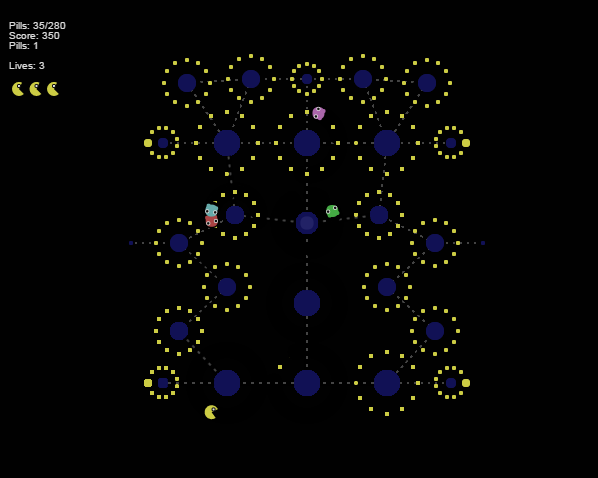
\includegraphics[width=0.9\textwidth]{pacman}
    \caption{A screenshot from the game}
    \label{fig:pacman}
\end{figure}

\section{The game}
The implementation described here is a port of my earlier clone of the game, which was written in Links\cite{links_site}, a functional language.
%This provides an interesting comparison

The mechanics of the game are slightly changed compared to the original. The maze of corridors is replaced by a maze of ``planets'', which are connected to each other. Pac-Man and the ghosts are in constant motion, as they orbit the planets, because there are no walls and 90-degree turns, which can stop them. Figure \ref{fig:pacman} shows a screen shot from the gameplay.

\subsection{Main loop}\label{sub:main_loop}
A typical game loop in a modern JavaScript game\cite{mdn_game_anatomy} relies on the \texttt{requestAnimationFrame} method\cite{mdn_requestanimationframe}. This method takes a single argument, which is a function callback. This function is invoked by the browser before it repaints the contents of the window. Thus, it allows the game rendering to be synchronized with the browser.

The callback invoked by \texttt{requestAnimationFrame} receives a timestamp,
which specifies the time of the repaint event. Ideally and under the most common
circumstances this happens 60 times a second.

I implemented the game loop in Dual as follows\footnote{Only the essential parts are shown in the listing, for the complete implementation, see the \texttt{src/pillman.dual} file in the DVD attached to this thesis.}:
\begin{lstlisting}
-- [1] the amount of milliseconds between game state updates:
bind [tick-length 50]

-- the main loop function:
--[
    arguments:
        -- current game state:
        game-state 
        -- time of the last game state update:
        last-tick
        -- the time of the current invocation of the loop:
        current-time
]
bind [main-loop of [
    game-state
    last-tick
    current-time
    
    do [ 
        -- [2] schedule the next iteration of the loop
        -- using requestAnimationFrame:
        async [
            .[window requestAnimationFrame] 
            of [next-time
                main-loop[
                    game-state
                    last-tick
                    next-time
               ]
           ]
        ]
        
        -- the timestamp of the tick after the last tick:
        bind [next-tick +[last-tick tick-length]]
        
        -- counts how many state updates should be
        -- performed in this iteration:
        bind [tick-count 0]
        
        -- if the current time is past the timestamp 
        -- of the next tick, the above counter should be
        -- incremented; possibly more than by one,
        -- if the difference is a multiply of tick-length:
        if [>[current-time next-tick] do [
            bind [time-since-tick -[current-time last-tick]]
            mutate [
                tick-count
                .[math floor][
                    /[time-since-tick tick-length]
                 ]
           ]
        ] _]
        
        -- [3] perform the calculated amount of game state updates:
        bind [i 0]
        while [<[i tick-count] do [
            -- keep track of the time of the last tick:
            mutate [last-tick +[last-tick tick-length]]
        
            -- [4] invoke the function that updates the game-state:
            mutate [
                game-state
                main-game-logic[game-state input-queue]
            ]
            
            mutate [i +[i 1]]
        ]]
        
        -- [5] if there were game state updates, redraw game screen;
        -- else do nothing:
        if [>[tick-count 0]
            draw[
                game-state
                current-time
                .[window performance now]!
            ]
            _
        ]
    ]
]]
\end{lstlisting}

The places in the above listing that require closer examination are marked with comments that contain a number in brackets, such as \texttt{[1]}. These comments are placed above the first line of the important fragment.

Each item on the below numbered list refers to the appropriately marked piece of code, as in 1. refers to \texttt{[1]}, 2. refers to \texttt{[2]} and so on:
\begin{enumerate}
\item The global variable \texttt{tick-length} is set to 50. It determines the frequency of game updates. 50 milliseconds translates to 20 Hz or 20 \acrshort{fps} (\acrlong{fps}). It turns out that the value of this variable very significantly determines the performance of the application and influences it in interesting ways, described later in ths chapter.

\item The first thing that happens in the main loop is a call to the \texttt{async} primitive, which schedules the next call to the main loop to happen in the next animation frame. This asynchronous recursive invocation ensures that the simulation runs continuously. The last argument to the next main loop invocation is \texttt{next-time}. It contains the timestamp of the next frame, provided by \texttt{requestAnimationFrame}.

\item The while loop performs game state updates. The longer the period since the last call to main loop, the more times it will execute.
\item The game state updates are performed by the \texttt{main-game-logic} function.
\item Drawing happens only if there were game state updates in the current main loop iteration. Otherwise a frame is essentially dropped.
\end{enumerate}

\section{Performance}
I encountered significant problems with performance of the application. In order to avoid unnecessary inflation of the volume of this thesis, I will not go into details, but outline the main points that explain the issues.

The game showed problems with performance fairly early into the implementation. Initially I set the value of the \texttt{tick-length} variable to 16.67 (milliseconds), to achieve a frame rate of 60 \acrshort{fps}. When I it with the \texttt{draw} function redrawing every yellow dot on the screen every frame, it rendered the application unresponsive.

In order to make the game run smoothly, I had to introduce an optimization where only the changed portion of the screen was redrawn each frame. I also had to decrease the value of \texttt{tick-length}, lowering the expected frame rate. This turned out to be different for different browsers.

For Chrome the value of \texttt{tick-length}, which allowed the game to run smoothly was 50. This means that an updates were happening every 50 milliseconds or at a frame rate of 20 \acrshort{fps}. Lower values caused the frame rate to destabilize and drop significantly on average.

In Firefox the application ran smoothly when \texttt{tick-length} was set to 75. This gives a frame rate of about 13 \acrshort{fps}. The performance in this browser was overall significantly worse than in Chrome.

I investigated the reason for the slow performance and the difference between Chrome and Firefox browsers with their built-in profilers. This showed that the slowdowns were caused by JavaScript's garbage collector, which was cleaning up large amounts of memory very often, thus pausing the execution.

The reason for this lies in the simple architecture of the interpreter. It works by recursively invoking a function that evaluates an expression. First the topmost expression (the root of the syntax tree) is evaluated. Then its each of its arguments, which are themselves expressions that have other expressions as arguments. This quickly results in a big tree of recursive calls on the call stack.

While the function that evaluates an expression is running, JavaScript's event loop is blocked, preventing any events from being handled and any other code from running.

Moreover, each of the stack frames contains references to various data, even though most of it is not relevant. But since it is referenced, the garbage collector cannot release the memory that the data takes up.

The collection can happen only when a whole syntax tree is evaluated and the stack is again empty. 

%happens when an asynchronous function is invoked, such as \texttt{requestAnimationFrame}, as at that point the call stack is empty.

The more calls in a single frame to the function that updates the game state, the more garbage to collect. This results in the collection pauses being longer. Because of that the frame rate drops.

The different patterns between Firefox and Chrome are caused by different garbage collection strategies\cite{mdn_mm, browser_gc}.

The general pattern seems to be that in Chrome the collections are more frequent, regular and predictable than in Firefox, which results in better performance, higher frame rate and smoother appearance of the game. 

%Figure \ref{fig:profiling2} contains four numbered samples from profiler outputs. They are aligned and scaled to match and were generated over the same span of time, a little less than 3 seconds. The part that is shown is 
%\begin{enumerate}
%\item Output from Firefox when the frame rate was low and unstable.
%\item Output from Firefox when the frame rate was smooth.
%\item Output from Chrome
%\item Output from Chrome
%\end{enumerate}
% two first  They are aligned with each other.  illustrates the general tendency
%
%\begin{figure}[h!]
%    \centering 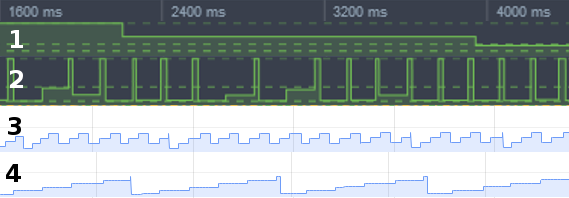
\includegraphics[width=0.9\textwidth]{profiling2}
%    \caption{Comparison of Firefox' and Chrome's profiler outputs}
%    \label{fig:profiling2}
%\end{figure}

%interpreter is blocking the event loop.  There's a lot of intermediate objects created that have to be garbage collected.

\section{Possible improvements}
To fix the described performance issues, the language's interpreter should be implemented in a way that takes into account the characteristics of the host language's environment. In case of JavaScript some of these are:
\begin{itemize}
\item The event-loop-based concurrency model. In JavaScript an iteration of event loop should run as fast as possible to achieve the best performance. 

An interpreter should not block the loop by recursive evaluation. The evaluation function should instead be interruptible. This could be achieved in multiple ways. One, which I experimented with\footnote{The file \texttt{dist/iterative-evaluate.js} contains an implementation of \texttt{evaluate} function that was used in earlier prototypes of the interpreter.}, is transforming the function into an iterative version by emulating the call stack. In this implementation, the function contains a variable that holds the stack frames for its own recursive invocations.

The function can thus pause evaluation between calls to itself, which should be asynchronous (similarly to the \texttt{main-loop} described in Section \ref{main_loop}) and not recursive. This releases the event loop.

Explicit control of the call stack allows trivial implementation of debugging facilities, since evaluation can now be paused at any time.

\item Automatic memory management with a garbage collector. An interpreter should create as little garbage as possible, should be free of memory leaks and possibly should manage memory ``manually'', using object pools or similar patterns.
\end{itemize}

An entirely different approach to improve performance would be compilation of the language to bytecode, straight to JavaScript or even to asm.js, a highly-optimizable low-level subset of JavaScript\cite{asmjs_spec}. 

Interruptable eval

Continuation-passing style State machine Anyway, explicit stack

Additional benefits: can pause and debug the application, step through can
record the state and rewind

\section{Conclusion}
Dynamic languages with a garbage collector allow a programmer to write code without worrying much about memory management or other low level considerations. But when it comes to performance and robustness this approach shows its downsides very quickly. 

The performance issues that I have encountered when implementing the Pac-Man clone, which are described in this chapter are very much related to the characteristics of the JavaScript environment. Notably the event loop and the garbage collector, which has different implementations with varying performance profiles across browsers. This shows in the performance differences when comparing different web browsers.

An interpreted language implemented without caring about low-level mechanisms, such as memory management is not suitable for writing non-trivial, performance-intensive applications, such as simulations or computer games.

This case study shows one of the disadvantages of exploratory programming.
